% Options for packages loaded elsewhere
\PassOptionsToPackage{unicode}{hyperref}
\PassOptionsToPackage{hyphens}{url}
%
\documentclass[
]{article}
\usepackage{amsmath,amssymb}
\usepackage{iftex}
\ifPDFTeX
  \usepackage[T1]{fontenc}
  \usepackage[utf8]{inputenc}
  \usepackage{textcomp} % provide euro and other symbols
\else % if luatex or xetex
  \usepackage{unicode-math} % this also loads fontspec
  \defaultfontfeatures{Scale=MatchLowercase}
  \defaultfontfeatures[\rmfamily]{Ligatures=TeX,Scale=1}
\fi
\usepackage{lmodern}
\ifPDFTeX\else
  % xetex/luatex font selection
\fi
% Use upquote if available, for straight quotes in verbatim environments
\IfFileExists{upquote.sty}{\usepackage{upquote}}{}
\IfFileExists{microtype.sty}{% use microtype if available
  \usepackage[]{microtype}
  \UseMicrotypeSet[protrusion]{basicmath} % disable protrusion for tt fonts
}{}
\makeatletter
\@ifundefined{KOMAClassName}{% if non-KOMA class
  \IfFileExists{parskip.sty}{%
    \usepackage{parskip}
  }{% else
    \setlength{\parindent}{0pt}
    \setlength{\parskip}{6pt plus 2pt minus 1pt}}
}{% if KOMA class
  \KOMAoptions{parskip=half}}
\makeatother
\usepackage{xcolor}
\usepackage[margin=1in]{geometry}
\usepackage{color}
\usepackage{fancyvrb}
\newcommand{\VerbBar}{|}
\newcommand{\VERB}{\Verb[commandchars=\\\{\}]}
\DefineVerbatimEnvironment{Highlighting}{Verbatim}{commandchars=\\\{\}}
% Add ',fontsize=\small' for more characters per line
\usepackage{framed}
\definecolor{shadecolor}{RGB}{248,248,248}
\newenvironment{Shaded}{\begin{snugshade}}{\end{snugshade}}
\newcommand{\AlertTok}[1]{\textcolor[rgb]{0.94,0.16,0.16}{#1}}
\newcommand{\AnnotationTok}[1]{\textcolor[rgb]{0.56,0.35,0.01}{\textbf{\textit{#1}}}}
\newcommand{\AttributeTok}[1]{\textcolor[rgb]{0.13,0.29,0.53}{#1}}
\newcommand{\BaseNTok}[1]{\textcolor[rgb]{0.00,0.00,0.81}{#1}}
\newcommand{\BuiltInTok}[1]{#1}
\newcommand{\CharTok}[1]{\textcolor[rgb]{0.31,0.60,0.02}{#1}}
\newcommand{\CommentTok}[1]{\textcolor[rgb]{0.56,0.35,0.01}{\textit{#1}}}
\newcommand{\CommentVarTok}[1]{\textcolor[rgb]{0.56,0.35,0.01}{\textbf{\textit{#1}}}}
\newcommand{\ConstantTok}[1]{\textcolor[rgb]{0.56,0.35,0.01}{#1}}
\newcommand{\ControlFlowTok}[1]{\textcolor[rgb]{0.13,0.29,0.53}{\textbf{#1}}}
\newcommand{\DataTypeTok}[1]{\textcolor[rgb]{0.13,0.29,0.53}{#1}}
\newcommand{\DecValTok}[1]{\textcolor[rgb]{0.00,0.00,0.81}{#1}}
\newcommand{\DocumentationTok}[1]{\textcolor[rgb]{0.56,0.35,0.01}{\textbf{\textit{#1}}}}
\newcommand{\ErrorTok}[1]{\textcolor[rgb]{0.64,0.00,0.00}{\textbf{#1}}}
\newcommand{\ExtensionTok}[1]{#1}
\newcommand{\FloatTok}[1]{\textcolor[rgb]{0.00,0.00,0.81}{#1}}
\newcommand{\FunctionTok}[1]{\textcolor[rgb]{0.13,0.29,0.53}{\textbf{#1}}}
\newcommand{\ImportTok}[1]{#1}
\newcommand{\InformationTok}[1]{\textcolor[rgb]{0.56,0.35,0.01}{\textbf{\textit{#1}}}}
\newcommand{\KeywordTok}[1]{\textcolor[rgb]{0.13,0.29,0.53}{\textbf{#1}}}
\newcommand{\NormalTok}[1]{#1}
\newcommand{\OperatorTok}[1]{\textcolor[rgb]{0.81,0.36,0.00}{\textbf{#1}}}
\newcommand{\OtherTok}[1]{\textcolor[rgb]{0.56,0.35,0.01}{#1}}
\newcommand{\PreprocessorTok}[1]{\textcolor[rgb]{0.56,0.35,0.01}{\textit{#1}}}
\newcommand{\RegionMarkerTok}[1]{#1}
\newcommand{\SpecialCharTok}[1]{\textcolor[rgb]{0.81,0.36,0.00}{\textbf{#1}}}
\newcommand{\SpecialStringTok}[1]{\textcolor[rgb]{0.31,0.60,0.02}{#1}}
\newcommand{\StringTok}[1]{\textcolor[rgb]{0.31,0.60,0.02}{#1}}
\newcommand{\VariableTok}[1]{\textcolor[rgb]{0.00,0.00,0.00}{#1}}
\newcommand{\VerbatimStringTok}[1]{\textcolor[rgb]{0.31,0.60,0.02}{#1}}
\newcommand{\WarningTok}[1]{\textcolor[rgb]{0.56,0.35,0.01}{\textbf{\textit{#1}}}}
\usepackage{graphicx}
\makeatletter
\def\maxwidth{\ifdim\Gin@nat@width>\linewidth\linewidth\else\Gin@nat@width\fi}
\def\maxheight{\ifdim\Gin@nat@height>\textheight\textheight\else\Gin@nat@height\fi}
\makeatother
% Scale images if necessary, so that they will not overflow the page
% margins by default, and it is still possible to overwrite the defaults
% using explicit options in \includegraphics[width, height, ...]{}
\setkeys{Gin}{width=\maxwidth,height=\maxheight,keepaspectratio}
% Set default figure placement to htbp
\makeatletter
\def\fps@figure{htbp}
\makeatother
\setlength{\emergencystretch}{3em} % prevent overfull lines
\providecommand{\tightlist}{%
  \setlength{\itemsep}{0pt}\setlength{\parskip}{0pt}}
\setcounter{secnumdepth}{-\maxdimen} % remove section numbering
\usepackage{fontspec}
\setmainfont{Times New Roman}
\usepackage{ctex}
\ifLuaTeX
  \usepackage{selnolig}  % disable illegal ligatures
\fi
\usepackage{bookmark}
\IfFileExists{xurl.sty}{\usepackage{xurl}}{} % add URL line breaks if available
\urlstyle{same}
\hypersetup{
  pdftitle={Mathematical practice final exam 2025},
  pdfauthor={黄舟翔 3220103606},
  hidelinks,
  pdfcreator={LaTeX via pandoc}}

\title{Mathematical practice final exam 2025}
\author{黄舟翔 3220103606}
\date{2025-07-02}

\begin{document}
\maketitle

\begin{verbatim}
## Warning: 程序包'tidyverse'是用R版本4.4.3 来建造的
\end{verbatim}

\begin{verbatim}
## Warning: 程序包'ggplot2'是用R版本4.4.3 来建造的
\end{verbatim}

\begin{verbatim}
## Warning: 程序包'tibble'是用R版本4.4.3 来建造的
\end{verbatim}

\begin{verbatim}
## Warning: 程序包'tidyr'是用R版本4.4.3 来建造的
\end{verbatim}

\begin{verbatim}
## Warning: 程序包'readr'是用R版本4.4.3 来建造的
\end{verbatim}

\begin{verbatim}
## Warning: 程序包'purrr'是用R版本4.4.3 来建造的
\end{verbatim}

\begin{verbatim}
## Warning: 程序包'dplyr'是用R版本4.4.3 来建造的
\end{verbatim}

\begin{verbatim}
## Warning: 程序包'stringr'是用R版本4.4.3 来建造的
\end{verbatim}

\begin{verbatim}
## Warning: 程序包'forcats'是用R版本4.4.3 来建造的
\end{verbatim}

\begin{verbatim}
## Warning: 程序包'lubridate'是用R版本4.4.3 来建造的
\end{verbatim}

\begin{verbatim}
## Warning: 程序包'Ecdat'是用R版本4.4.3 来建造的
\end{verbatim}

\begin{verbatim}
## Warning: 程序包'Ecfun'是用R版本4.4.3 来建造的
\end{verbatim}

\subsection{1.}\label{section}

Find the inverse of the following matrix and verify it using the
\texttt{all.equal()} function. \[
\left(\begin{array}{cccc}
9 & 4 & 12 & 2 \\
5 & 0 & 7 & 9 \\
2 & 6 & 8 & 0 \\
9 & 2 & 9 & 11
\end{array}\right) 
\] 用以下代码解决：

\begin{Shaded}
\begin{Highlighting}[]
\CommentTok{\# Define the original matrix}
\NormalTok{A }\OtherTok{\textless{}{-}} \FunctionTok{matrix}\NormalTok{(}\FunctionTok{c}\NormalTok{(}\DecValTok{9}\NormalTok{, }\DecValTok{5}\NormalTok{, }\DecValTok{2}\NormalTok{, }\DecValTok{9}\NormalTok{,}
              \DecValTok{4}\NormalTok{, }\DecValTok{0}\NormalTok{, }\DecValTok{6}\NormalTok{, }\DecValTok{2}\NormalTok{,}
              \DecValTok{12}\NormalTok{, }\DecValTok{7}\NormalTok{, }\DecValTok{8}\NormalTok{, }\DecValTok{9}\NormalTok{,}
              \DecValTok{2}\NormalTok{, }\DecValTok{9}\NormalTok{, }\DecValTok{0}\NormalTok{, }\DecValTok{11}\NormalTok{), }
            \AttributeTok{nrow =} \DecValTok{4}\NormalTok{, }\AttributeTok{byrow =} \ConstantTok{TRUE}\NormalTok{)}

\CommentTok{\# Compute the inverse}
\NormalTok{A\_inv }\OtherTok{\textless{}{-}} \FunctionTok{solve}\NormalTok{(A)}

\CommentTok{\# Print the inverse (rounded for clarity)}
\FunctionTok{print}\NormalTok{(}\StringTok{"Inverse Matrix:"}\NormalTok{)}
\end{Highlighting}
\end{Shaded}

\begin{verbatim}
## [1] "Inverse Matrix:"
\end{verbatim}

\begin{Shaded}
\begin{Highlighting}[]
\FunctionTok{print}\NormalTok{(}\FunctionTok{round}\NormalTok{(A\_inv, }\DecValTok{5}\NormalTok{))}
\end{Highlighting}
\end{Shaded}

\begin{verbatim}
##          [,1]     [,2]     [,3]     [,4]
## [1,]  0.08571 -0.14286  0.08571 -0.11429
## [2,] -0.26000 -0.30000  0.29000  0.03000
## [3,] -0.12286  0.17143  0.02714  0.04714
## [4,]  0.19714  0.27143 -0.25286  0.08714
\end{verbatim}

\begin{Shaded}
\begin{Highlighting}[]
\CommentTok{\# Verification: Multiply A by A\_inv}
\NormalTok{product }\OtherTok{\textless{}{-}}\NormalTok{ A }\SpecialCharTok{\%*\%}\NormalTok{ A\_inv}

\CommentTok{\# Check if the product is the identity matrix}
\NormalTok{is\_identity }\OtherTok{\textless{}{-}} \FunctionTok{all.equal}\NormalTok{(product, }\FunctionTok{diag}\NormalTok{(}\DecValTok{4}\NormalTok{))}

\CommentTok{\# Print verification result}
\FunctionTok{print}\NormalTok{(}\StringTok{"Verification Result:"}\NormalTok{)}
\end{Highlighting}
\end{Shaded}

\begin{verbatim}
## [1] "Verification Result:"
\end{verbatim}

\begin{Shaded}
\begin{Highlighting}[]
\FunctionTok{print}\NormalTok{(is\_identity)}
\end{Highlighting}
\end{Shaded}

\begin{verbatim}
## [1] TRUE
\end{verbatim}

\subsection{2.}\label{section-1}

Execute the following lines which create two vectors of random integers
which are chosen with replacement from the integers
\(0, 1, \dots , 999\). Both vectors have length 250.

\begin{Shaded}
\begin{Highlighting}[]
\NormalTok{xVec }\OtherTok{\textless{}{-}} \FunctionTok{sample}\NormalTok{(}\DecValTok{0}\SpecialCharTok{:}\DecValTok{999}\NormalTok{, }\DecValTok{250}\NormalTok{, }\AttributeTok{replace=}\NormalTok{T)}
\NormalTok{yVec }\OtherTok{\textless{}{-}} \FunctionTok{sample}\NormalTok{(}\DecValTok{0}\SpecialCharTok{:}\DecValTok{999}\NormalTok{, }\DecValTok{250}\NormalTok{, }\AttributeTok{replace=}\NormalTok{T)}
\end{Highlighting}
\end{Shaded}

\begin{enumerate}
\def\labelenumi{(\alph{enumi})}
\tightlist
\item
  Create the vector \((y_2 - x_1, \cdots, y_n - x_{n-1}).\)
\end{enumerate}

\begin{Shaded}
\begin{Highlighting}[]
\NormalTok{xVec }\OtherTok{\textless{}{-}} \FunctionTok{sample}\NormalTok{(}\DecValTok{0}\SpecialCharTok{:}\DecValTok{999}\NormalTok{, }\DecValTok{250}\NormalTok{, }\AttributeTok{replace =} \ConstantTok{TRUE}\NormalTok{)}
\NormalTok{yVec }\OtherTok{\textless{}{-}} \FunctionTok{sample}\NormalTok{(}\DecValTok{0}\SpecialCharTok{:}\DecValTok{999}\NormalTok{, }\DecValTok{250}\NormalTok{, }\AttributeTok{replace =} \ConstantTok{TRUE}\NormalTok{)}
\NormalTok{part\_a }\OtherTok{\textless{}{-}}\NormalTok{ yVec[}\SpecialCharTok{{-}}\DecValTok{1}\NormalTok{] }\SpecialCharTok{{-}}\NormalTok{ xVec[}\SpecialCharTok{{-}}\FunctionTok{length}\NormalTok{(xVec)]}
\end{Highlighting}
\end{Shaded}

\begin{enumerate}
\def\labelenumi{(\alph{enumi})}
\setcounter{enumi}{1}
\tightlist
\item
  Pick out the values in yVec which are \(> 600\).
\end{enumerate}

\begin{Shaded}
\begin{Highlighting}[]
\NormalTok{part\_b }\OtherTok{\textless{}{-}}\NormalTok{ yVec[yVec }\SpecialCharTok{\textgreater{}} \DecValTok{600}\NormalTok{]}
\FunctionTok{print}\NormalTok{(part\_b)}
\end{Highlighting}
\end{Shaded}

\begin{verbatim}
##   [1] 790 780 899 613 780 786 849 613 904 967 915 908 780 750 676 733 719 689
##  [19] 695 765 896 678 858 850 736 989 983 754 614 635 921 876 861 917 747 819
##  [37] 601 812 669 964 720 956 765 976 728 811 995 863 782 614 896 749 996 844
##  [55] 721 692 711 708 618 861 773 962 804 661 867 724 999 695 726 645 912 869
##  [73] 812 882 946 957 611 642 975 657 841 777 884 887 956 879 730 941 675 924
##  [91] 807 661 966 916 768 650 894 675 965 657
\end{verbatim}

\begin{enumerate}
\def\labelenumi{(\alph{enumi})}
\setcounter{enumi}{2}
\tightlist
\item
  What are the index positions in yVec of the values which are
  \(> 600\)?
\end{enumerate}

\begin{Shaded}
\begin{Highlighting}[]
\NormalTok{part\_c }\OtherTok{\textless{}{-}} \FunctionTok{which}\NormalTok{(yVec }\SpecialCharTok{\textgreater{}} \DecValTok{600}\NormalTok{)}
\NormalTok{part\_c}
\end{Highlighting}
\end{Shaded}

\begin{verbatim}
##   [1]   5   6   7   9  10  11  13  14  18  22  24  30  32  33  35  40  41  42
##  [19]  44  47  49  52  53  54  56  57  65  68  70  71  78  79  80  81  83  84
##  [37]  85  86  88  92  93  96  99 101 102 103 105 109 110 112 116 119 120 121
##  [55] 123 124 125 131 132 133 135 137 142 150 153 154 157 167 169 170 171 173
##  [73] 174 178 183 184 186 188 205 206 207 208 211 212 214 215 217 219 224 230
##  [91] 231 233 234 238 239 244 245 247 249 250
\end{verbatim}

\begin{enumerate}
\def\labelenumi{(\alph{enumi})}
\setcounter{enumi}{3}
\tightlist
\item
  Sort the numbers in the vector xVec in the order of increasing values
  in yVec.
\end{enumerate}

\begin{Shaded}
\begin{Highlighting}[]
\NormalTok{part\_d }\OtherTok{\textless{}{-}}\NormalTok{ xVec[}\FunctionTok{order}\NormalTok{(yVec)]}
\end{Highlighting}
\end{Shaded}

\begin{enumerate}
\def\labelenumi{(\alph{enumi})}
\setcounter{enumi}{4}
\tightlist
\item
  Pick out the elements in yVec at index positions
  \(1, 4, 7, 10, 13, \cdots\)
\end{enumerate}

\begin{Shaded}
\begin{Highlighting}[]
\NormalTok{indices }\OtherTok{\textless{}{-}} \FunctionTok{seq}\NormalTok{(}\DecValTok{1}\NormalTok{, }\FunctionTok{length}\NormalTok{(yVec), }\AttributeTok{by =} \DecValTok{3}\NormalTok{)}
\NormalTok{part\_e }\OtherTok{\textless{}{-}}\NormalTok{ yVec[indices]}
\NormalTok{part\_e}
\end{Highlighting}
\end{Shaded}

\begin{verbatim}
##  [1] 113 222 899 780 849 376 360 967 166 518 403  79 209 733 277 195 896 678  57
## [20] 466 421 369 354 614 295  92 876 480 601 669 435 489  38 165 811 108 863 614
## [39] 335 362 844 692 402 391 861  43 410 804 123 510 547 724 999  12 244 442 726
## [58] 546 158 882 551 957 102 267 289 151  91 382 975 777 884 956 730 338 343 294
## [77] 521 206  53 916 387 650 675 657
\end{verbatim}

\subsection{3.}\label{section-2}

For this problem we'll use the (built-in) dataset state.x77.

\begin{Shaded}
\begin{Highlighting}[]
\FunctionTok{data}\NormalTok{(state)}
\NormalTok{state.x77 }\OtherTok{\textless{}{-}} \FunctionTok{as\_tibble}\NormalTok{(state.x77, }\AttributeTok{rownames  =} \StringTok{\textquotesingle{}State\textquotesingle{}}\NormalTok{)}
\end{Highlighting}
\end{Shaded}

\begin{enumerate}
\def\labelenumi{\alph{enumi}.}
\tightlist
\item
  Select all the states having an income less than 4300, and calculate
  the average income of these states.
\end{enumerate}

\begin{Shaded}
\begin{Highlighting}[]
\NormalTok{low\_income\_states }\OtherTok{\textless{}{-}}\NormalTok{ state.x77 }\SpecialCharTok{\%\textgreater{}\%}
  \FunctionTok{filter}\NormalTok{(Income }\SpecialCharTok{\textless{}} \DecValTok{4300}\NormalTok{)}

\NormalTok{average\_income\_low }\OtherTok{\textless{}{-}} \FunctionTok{mean}\NormalTok{(low\_income\_states}\SpecialCharTok{$}\NormalTok{Income)}
\FunctionTok{cat}\NormalTok{(}\StringTok{"a. 收入低于4300的州平均收入为:"}\NormalTok{, }\FunctionTok{round}\NormalTok{(average\_income\_low, }\DecValTok{2}\NormalTok{), }\StringTok{"}\SpecialCharTok{\textbackslash{}n\textbackslash{}n}\StringTok{"}\NormalTok{)}
\end{Highlighting}
\end{Shaded}

\begin{verbatim}
## a. 收入低于4300的州平均收入为: 3830.6
\end{verbatim}

\begin{enumerate}
\def\labelenumi{\alph{enumi}.}
\setcounter{enumi}{1}
\tightlist
\item
  Sort the data by income and select the state with the highest income.
\end{enumerate}

\begin{Shaded}
\begin{Highlighting}[]
\NormalTok{highest\_income\_state }\OtherTok{\textless{}{-}}\NormalTok{ state.x77 }\SpecialCharTok{\%\textgreater{}\%}
  \FunctionTok{arrange}\NormalTok{(}\FunctionTok{desc}\NormalTok{(Income)) }\SpecialCharTok{\%\textgreater{}\%}
  \FunctionTok{slice}\NormalTok{(}\DecValTok{1}\NormalTok{)}
\FunctionTok{cat}\NormalTok{(}\StringTok{"b. 收入最高的州:}\SpecialCharTok{\textbackslash{}n}\StringTok{"}\NormalTok{)}
\end{Highlighting}
\end{Shaded}

\begin{verbatim}
## b. 收入最高的州:
\end{verbatim}

\begin{Shaded}
\begin{Highlighting}[]
\FunctionTok{print}\NormalTok{(highest\_income\_state)}
\end{Highlighting}
\end{Shaded}

\begin{verbatim}
## # A tibble: 1 x 9
##   State  Population Income Illiteracy `Life Exp` Murder `HS Grad` Frost   Area
##   <chr>       <dbl>  <dbl>      <dbl>      <dbl>  <dbl>     <dbl> <dbl>  <dbl>
## 1 Alaska        365   6315        1.5       69.3   11.3      66.7   152 566432
\end{verbatim}

\begin{Shaded}
\begin{Highlighting}[]
\FunctionTok{cat}\NormalTok{(}\StringTok{"}\SpecialCharTok{\textbackslash{}n}\StringTok{"}\NormalTok{)}
\end{Highlighting}
\end{Shaded}

\begin{enumerate}
\def\labelenumi{\alph{enumi}.}
\setcounter{enumi}{2}
\item
  Add a variable to the data frame which categorizes the size of
  population: \(<= 4500\) is \texttt{S}, \(> 4500\) is \texttt{L}.
\item
  Find out the average income and illiteracy of the two groups of
  states, distinguishing by whether the states are small or large.
\end{enumerate}

\begin{Shaded}
\begin{Highlighting}[]
\NormalTok{grouped\_stats }\OtherTok{\textless{}{-}}\NormalTok{ state\_data }\SpecialCharTok{\%\textgreater{}\%}
  \FunctionTok{group\_by}\NormalTok{(Pop\_Size) }\SpecialCharTok{\%\textgreater{}\%}
  \FunctionTok{summarise}\NormalTok{(}
    \AttributeTok{Avg\_Income =} \FunctionTok{mean}\NormalTok{(Income),}
    \AttributeTok{Avg\_Illiteracy =} \FunctionTok{mean}\NormalTok{(Illiteracy)}
\NormalTok{  )}
\FunctionTok{cat}\NormalTok{(}\StringTok{"d. 按人口规模分组的统计:}\SpecialCharTok{\textbackslash{}n}\StringTok{"}\NormalTok{)}
\end{Highlighting}
\end{Shaded}

\begin{verbatim}
## d. 按人口规模分组的统计:
\end{verbatim}

\begin{Shaded}
\begin{Highlighting}[]
\FunctionTok{print}\NormalTok{(grouped\_stats)}
\end{Highlighting}
\end{Shaded}

\begin{verbatim}
## # A tibble: 2 x 3
##   Pop_Size Avg_Income Avg_Illiteracy
##   <chr>         <dbl>          <dbl>
## 1 L             4608.           1.2 
## 2 S             4355.           1.16
\end{verbatim}

\subsection{4.}\label{section-3}

\begin{enumerate}
\def\labelenumi{\alph{enumi}.}
\tightlist
\item
  Write a function to simulate \texttt{n} observations of \((X_1, X_2)\)
  which follow the uniform distribution over the square
  \([0, 1] \times [0, 1]\).
\end{enumerate}

\begin{Shaded}
\begin{Highlighting}[]
\NormalTok{simulate\_points }\OtherTok{\textless{}{-}} \ControlFlowTok{function}\NormalTok{(n) \{}
  \CommentTok{\# 生成 n 个在 [0,1]x[0,1] 正方形内的均匀分布点}
\NormalTok{  x1 }\OtherTok{\textless{}{-}} \FunctionTok{runif}\NormalTok{(n, }\AttributeTok{min =} \DecValTok{0}\NormalTok{, }\AttributeTok{max =} \DecValTok{1}\NormalTok{)}
\NormalTok{  x2 }\OtherTok{\textless{}{-}} \FunctionTok{runif}\NormalTok{(n, }\AttributeTok{min =} \DecValTok{0}\NormalTok{, }\AttributeTok{max =} \DecValTok{1}\NormalTok{)}
  \FunctionTok{data.frame}\NormalTok{(}\AttributeTok{x1 =}\NormalTok{ x1, }\AttributeTok{x2 =}\NormalTok{ x2)}
\NormalTok{\}}
\end{Highlighting}
\end{Shaded}

\begin{enumerate}
\def\labelenumi{\alph{enumi}.}
\setcounter{enumi}{1}
\tightlist
\item
  Write a function to calculate the proportion of the observations that
  the distance between \((X_1, X_2)\) and the nearest edge is less than
  0.25, and the proportion of them with the distance to the nearest
  vertex less than 0.25.
\end{enumerate}

\begin{Shaded}
\begin{Highlighting}[]
\NormalTok{calculate\_proportions }\OtherTok{\textless{}{-}} \ControlFlowTok{function}\NormalTok{(points) \{}
  \CommentTok{\# 计算到最近边的距离}
\NormalTok{  dist\_to\_edges }\OtherTok{\textless{}{-}} \FunctionTok{with}\NormalTok{(points, }\FunctionTok{pmin}\NormalTok{(x1, }\DecValTok{1} \SpecialCharTok{{-}}\NormalTok{ x1, x2, }\DecValTok{1} \SpecialCharTok{{-}}\NormalTok{ x2))}
  
  \CommentTok{\# 计算到四个顶点的距离}
\NormalTok{  dist\_to\_corners }\OtherTok{\textless{}{-}} \FunctionTok{with}\NormalTok{(points, \{}
\NormalTok{    d1 }\OtherTok{\textless{}{-}} \FunctionTok{sqrt}\NormalTok{(x1}\SpecialCharTok{\^{}}\DecValTok{2} \SpecialCharTok{+}\NormalTok{ x2}\SpecialCharTok{\^{}}\DecValTok{2}\NormalTok{)          }\CommentTok{\# 到 (0,0) 的距离}
\NormalTok{    d2 }\OtherTok{\textless{}{-}} \FunctionTok{sqrt}\NormalTok{(x1}\SpecialCharTok{\^{}}\DecValTok{2} \SpecialCharTok{+}\NormalTok{ (}\DecValTok{1} \SpecialCharTok{{-}}\NormalTok{ x2)}\SpecialCharTok{\^{}}\DecValTok{2}\NormalTok{)    }\CommentTok{\# 到 (0,1) 的距离}
\NormalTok{    d3 }\OtherTok{\textless{}{-}} \FunctionTok{sqrt}\NormalTok{((}\DecValTok{1} \SpecialCharTok{{-}}\NormalTok{ x1)}\SpecialCharTok{\^{}}\DecValTok{2} \SpecialCharTok{+}\NormalTok{ x2}\SpecialCharTok{\^{}}\DecValTok{2}\NormalTok{)    }\CommentTok{\# 到 (1,0) 的距离}
\NormalTok{    d4 }\OtherTok{\textless{}{-}} \FunctionTok{sqrt}\NormalTok{((}\DecValTok{1} \SpecialCharTok{{-}}\NormalTok{ x1)}\SpecialCharTok{\^{}}\DecValTok{2} \SpecialCharTok{+}\NormalTok{ (}\DecValTok{1} \SpecialCharTok{{-}}\NormalTok{ x2)}\SpecialCharTok{\^{}}\DecValTok{2}\NormalTok{) }\CommentTok{\# 到 (1,1) 的距离}
    \FunctionTok{pmin}\NormalTok{(d1, d2, d3, d4)             }\CommentTok{\# 取最小值得到最近顶点距离}
\NormalTok{  \})}
  
  \CommentTok{\# 计算比例}
\NormalTok{  prop\_edge }\OtherTok{\textless{}{-}} \FunctionTok{mean}\NormalTok{(dist\_to\_edges }\SpecialCharTok{\textless{}} \FloatTok{0.25}\NormalTok{)}
\NormalTok{  prop\_vertex }\OtherTok{\textless{}{-}} \FunctionTok{mean}\NormalTok{(dist\_to\_corners }\SpecialCharTok{\textless{}} \FloatTok{0.25}\NormalTok{)}
  
  \FunctionTok{list}\NormalTok{(}\AttributeTok{prop\_edge =}\NormalTok{ prop\_edge, }\AttributeTok{prop\_vertex =}\NormalTok{ prop\_vertex)}
\NormalTok{\}}

\CommentTok{\# 测试函数}
\FunctionTok{set.seed}\NormalTok{(}\DecValTok{123}\NormalTok{) }\CommentTok{\# 确保结果可重现}
\NormalTok{n }\OtherTok{\textless{}{-}} \DecValTok{10000}    \CommentTok{\# 样本大小}

\CommentTok{\# 模拟数据点}
\NormalTok{points\_df }\OtherTok{\textless{}{-}} \FunctionTok{simulate\_points}\NormalTok{(n)}

\CommentTok{\# 计算比例}
\NormalTok{results }\OtherTok{\textless{}{-}} \FunctionTok{calculate\_proportions}\NormalTok{(points\_df)}

\CommentTok{\# 输出结果}
\FunctionTok{cat}\NormalTok{(}\StringTok{"到最近边的距离 \textless{} 0.25 的比例:"}\NormalTok{, }\FunctionTok{round}\NormalTok{(results}\SpecialCharTok{$}\NormalTok{prop\_edge, }\DecValTok{4}\NormalTok{), }\StringTok{"}\SpecialCharTok{\textbackslash{}n}\StringTok{"}\NormalTok{)}
\end{Highlighting}
\end{Shaded}

\begin{verbatim}
## 到最近边的距离 < 0.25 的比例: 0.7493
\end{verbatim}

\begin{Shaded}
\begin{Highlighting}[]
\FunctionTok{cat}\NormalTok{(}\StringTok{"到最近顶点的距离 \textless{} 0.25 的比例:"}\NormalTok{, }\FunctionTok{round}\NormalTok{(results}\SpecialCharTok{$}\NormalTok{prop\_vertex, }\DecValTok{4}\NormalTok{), }\StringTok{"}\SpecialCharTok{\textbackslash{}n}\StringTok{"}\NormalTok{)}
\end{Highlighting}
\end{Shaded}

\begin{verbatim}
## 到最近顶点的距离 < 0.25 的比例: 0.1948
\end{verbatim}

\subsection{5.}\label{section-4}

To estimate \(\pi\) with a Monte Carlo simulation, we draw the unit
circle inside the unit square, the ratio of the area of the circle to
the area of the square will be \(\pi / 4\). Then shot \(K\) arrows at
the square, roughly \(K * \pi / 4\) should have fallen inside the
circle. So if now you shoot \(N\) arrows at the square, and \(M\) fall
inside the circle, you have the following relationship
\(M = N * \pi / 4\). You can thus compute \(\pi\) like so:
\(\pi = 4 * M / N\). The more arrows \(N\) you throw at the square, the
better approximation of \(\pi\) you'll have.

\begin{Shaded}
\begin{Highlighting}[]
\NormalTok{n }\OtherTok{\textless{}{-}} \DecValTok{10000}

\FunctionTok{set.seed}\NormalTok{(}\DecValTok{1}\NormalTok{)}
\NormalTok{points }\OtherTok{\textless{}{-}} \FunctionTok{tibble}\NormalTok{(}\StringTok{"x"} \OtherTok{=} \FunctionTok{runif}\NormalTok{(n), }\StringTok{"y"} \OtherTok{=} \FunctionTok{runif}\NormalTok{(n))}
\end{Highlighting}
\end{Shaded}

Now, to know if a point is inside the unit circle, we need to check
whether \(x^2 + y^2 < 1\). Let's add a new column to the points tibble,
called \texttt{inside} equal to \texttt{1} if the point is inside the
unit circle and \texttt{0} if not:

\begin{Shaded}
\begin{Highlighting}[]
\NormalTok{points }\OtherTok{\textless{}{-}}\NormalTok{ points }\SpecialCharTok{|\textgreater{}}
\FunctionTok{mutate}\NormalTok{(}\AttributeTok{inside =} \FunctionTok{map2\_dbl}\NormalTok{(}\AttributeTok{.x =}\NormalTok{ x, }\AttributeTok{.y =}\NormalTok{ y, }\SpecialCharTok{\textasciitilde{}}\FunctionTok{ifelse}\NormalTok{(.x}\SpecialCharTok{**}\DecValTok{2} \SpecialCharTok{+}\NormalTok{ .y}\SpecialCharTok{**}\DecValTok{2} \SpecialCharTok{\textless{}} \DecValTok{1}\NormalTok{, }\DecValTok{1}\NormalTok{, }\DecValTok{0}\NormalTok{))) }\SpecialCharTok{|\textgreater{}}
\FunctionTok{rowid\_to\_column}\NormalTok{(}\StringTok{"N"}\NormalTok{)}
\end{Highlighting}
\end{Shaded}

\begin{enumerate}
\def\labelenumi{\alph{enumi}.}
\tightlist
\item
  Compute the estimation of \(\pi\) at each row, by computing the
  cumulative sum of the 1's in the \texttt{inside} column and dividing
  that by the current value of \texttt{N} column:
\end{enumerate}

\begin{Shaded}
\begin{Highlighting}[]
\NormalTok{points }\OtherTok{\textless{}{-}}\NormalTok{ points }\SpecialCharTok{\%\textgreater{}\%}
  \FunctionTok{mutate}\NormalTok{(}
    \AttributeTok{cum\_inside =} \FunctionTok{cumsum}\NormalTok{(inside),  }\CommentTok{\# 累积落入圆内的点数}
    \AttributeTok{pi\_estimate =} \DecValTok{4} \SpecialCharTok{*}\NormalTok{ cum\_inside }\SpecialCharTok{/}\NormalTok{ N  }\CommentTok{\# π的累积估计值}
\NormalTok{  )}
\FunctionTok{tail}\NormalTok{(points, }\DecValTok{5}\NormalTok{)}
\end{Highlighting}
\end{Shaded}

\begin{verbatim}
## # A tibble: 5 x 6
##       N     x     y inside cum_inside pi_estimate
##   <int> <dbl> <dbl>  <dbl>      <dbl>       <dbl>
## 1  9996 0.732 0.788      0       7824        3.13
## 2  9997 0.499 0.814      1       7825        3.13
## 3  9998 0.503 0.478      1       7826        3.13
## 4  9999 0.568 0.602      1       7827        3.13
## 5 10000 0.653 0.111      1       7828        3.13
\end{verbatim}

\begin{enumerate}
\def\labelenumi{\alph{enumi}.}
\setcounter{enumi}{1}
\tightlist
\item
  Plot the estimates of \(\pi\) against \texttt{N}.
\end{enumerate}

\begin{Shaded}
\begin{Highlighting}[]
\NormalTok{final\_pi }\OtherTok{\textless{}{-}} \FunctionTok{last}\NormalTok{(points}\SpecialCharTok{$}\NormalTok{pi\_estimate)}
\FunctionTok{cat}\NormalTok{(}\StringTok{"最终π估计值:"}\NormalTok{, }\FunctionTok{round}\NormalTok{(final\_pi, }\DecValTok{6}\NormalTok{), }\StringTok{"}\SpecialCharTok{\textbackslash{}n}\StringTok{"}\NormalTok{)}
\end{Highlighting}
\end{Shaded}

\begin{verbatim}
## 最终π估计值: 3.1312
\end{verbatim}

\begin{Shaded}
\begin{Highlighting}[]
\CommentTok{\# b. 绘制π估计值随N变化的曲线（不使用对数坐标）}
\FunctionTok{ggplot}\NormalTok{(points, }\FunctionTok{aes}\NormalTok{(}\AttributeTok{x =}\NormalTok{ N, }\AttributeTok{y =}\NormalTok{ pi\_estimate)) }\SpecialCharTok{+}
  \FunctionTok{geom\_line}\NormalTok{(}\AttributeTok{color =} \StringTok{"blue"}\NormalTok{, }\AttributeTok{alpha =} \FloatTok{0.7}\NormalTok{) }\SpecialCharTok{+}
  \FunctionTok{geom\_hline}\NormalTok{(}\AttributeTok{yintercept =}\NormalTok{ pi, }\AttributeTok{color =} \StringTok{"red"}\NormalTok{, }\AttributeTok{linetype =} \StringTok{"dashed"}\NormalTok{, }\AttributeTok{size =} \DecValTok{1}\NormalTok{) }\SpecialCharTok{+}
  \FunctionTok{labs}\NormalTok{(}\AttributeTok{title =} \StringTok{"Monte Carlo method for estimating the value of π"}\NormalTok{,}
       \AttributeTok{subtitle =} \FunctionTok{paste}\NormalTok{(}\StringTok{"Final estimate ="}\NormalTok{, }\FunctionTok{round}\NormalTok{(final\_pi, }\DecValTok{6}\NormalTok{), }\StringTok{"real ="}\NormalTok{, }\FunctionTok{round}\NormalTok{(pi, }\DecValTok{6}\NormalTok{)),}
       \AttributeTok{x =} \StringTok{"Sample size (N)"}\NormalTok{,}
       \AttributeTok{y =} \StringTok{"π estimated value"}\NormalTok{) }\SpecialCharTok{+}
  \FunctionTok{theme\_minimal}\NormalTok{() }\SpecialCharTok{+}
  \CommentTok{\# 添加平滑曲线显示趋势}
  \FunctionTok{geom\_smooth}\NormalTok{(}\AttributeTok{method =} \StringTok{"loess"}\NormalTok{, }\AttributeTok{se =} \ConstantTok{FALSE}\NormalTok{, }\AttributeTok{color =} \StringTok{"darkblue"}\NormalTok{, }\AttributeTok{size =} \FloatTok{0.8}\NormalTok{) }\SpecialCharTok{+}
  \CommentTok{\# 添加说明文本}
  \FunctionTok{annotate}\NormalTok{(}\StringTok{"text"}\NormalTok{, }\AttributeTok{x =}\NormalTok{ n }\SpecialCharTok{*} \FloatTok{0.7}\NormalTok{, }\AttributeTok{y =}\NormalTok{ pi }\SpecialCharTok{+} \FloatTok{0.1}\NormalTok{, }
           \AttributeTok{label =} \StringTok{"The true value of π"}\NormalTok{, }\AttributeTok{color =} \StringTok{"red"}\NormalTok{, }\AttributeTok{size =} \DecValTok{4}\NormalTok{) }\SpecialCharTok{+}
  \CommentTok{\# 限制y轴范围以更好地显示收敛}
  \FunctionTok{coord\_cartesian}\NormalTok{(}\AttributeTok{ylim =} \FunctionTok{c}\NormalTok{(}\FloatTok{2.8}\NormalTok{, }\FloatTok{3.5}\NormalTok{))}
\end{Highlighting}
\end{Shaded}

\begin{verbatim}
## Warning: Using `size` aesthetic for lines was deprecated in ggplot2 3.4.0.
## i Please use `linewidth` instead.
## This warning is displayed once every 8 hours.
## Call `lifecycle::last_lifecycle_warnings()` to see where this warning was
## generated.
\end{verbatim}

\begin{verbatim}
## `geom_smooth()` using formula = 'y ~ x'
\end{verbatim}

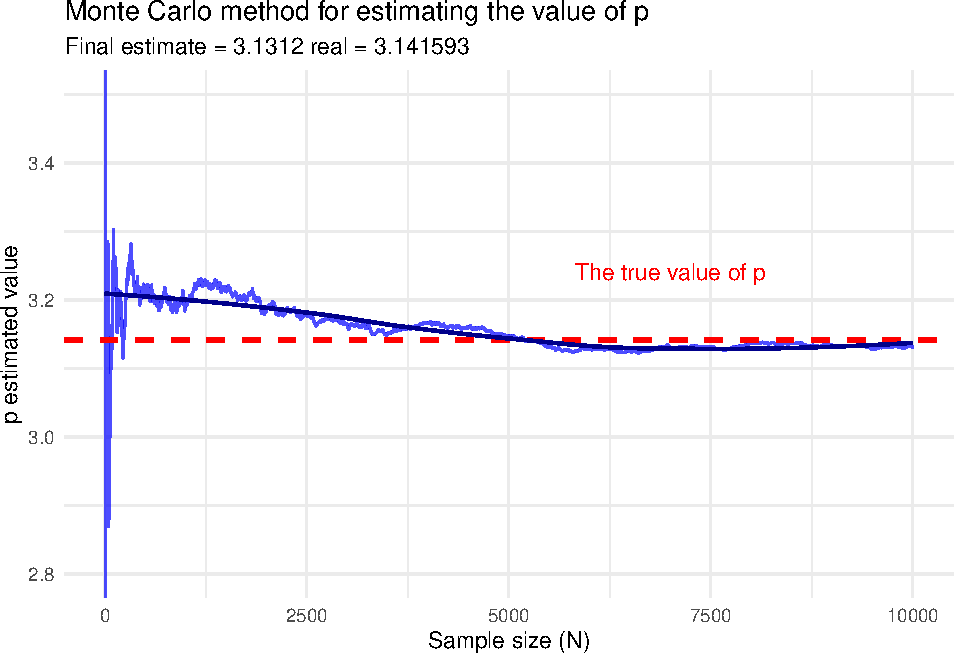
\includegraphics{final2025_files/figure-latex/unnamed-chunk-19-1.pdf}

\subsection{6.}\label{section-5}

Mortality rates per 100,000 from male suicides for a number of age
groups and a number of countries are given in the following data frame.

\begin{Shaded}
\begin{Highlighting}[]
\NormalTok{suicrates }\OtherTok{\textless{}{-}} \FunctionTok{tibble}\NormalTok{(}\AttributeTok{Country =} \FunctionTok{c}\NormalTok{(}\StringTok{\textquotesingle{}Canada\textquotesingle{}}\NormalTok{, }\StringTok{\textquotesingle{}Israel\textquotesingle{}}\NormalTok{, }\StringTok{\textquotesingle{}Japan\textquotesingle{}}\NormalTok{, }\StringTok{\textquotesingle{}Austria\textquotesingle{}}\NormalTok{, }\StringTok{\textquotesingle{}France\textquotesingle{}}\NormalTok{, }\StringTok{\textquotesingle{}Germany\textquotesingle{}}\NormalTok{,}
\StringTok{\textquotesingle{}Hungary\textquotesingle{}}\NormalTok{, }\StringTok{\textquotesingle{}Italy\textquotesingle{}}\NormalTok{, }\StringTok{\textquotesingle{}Netherlands\textquotesingle{}}\NormalTok{, }\StringTok{\textquotesingle{}Poland\textquotesingle{}}\NormalTok{, }\StringTok{\textquotesingle{}Spain\textquotesingle{}}\NormalTok{, }\StringTok{\textquotesingle{}Sweden\textquotesingle{}}\NormalTok{, }\StringTok{\textquotesingle{}Switzerland\textquotesingle{}}\NormalTok{, }\StringTok{\textquotesingle{}UK\textquotesingle{}}\NormalTok{, }\StringTok{\textquotesingle{}USA\textquotesingle{}}\NormalTok{), }
\AttributeTok{Age25.34 =} \FunctionTok{c}\NormalTok{(}\DecValTok{22}\NormalTok{,  }\DecValTok{9}\NormalTok{, }\DecValTok{22}\NormalTok{, }\DecValTok{29}\NormalTok{, }\DecValTok{16}\NormalTok{, }\DecValTok{28}\NormalTok{, }\DecValTok{48}\NormalTok{,  }\DecValTok{7}\NormalTok{,  }\DecValTok{8}\NormalTok{, }\DecValTok{26}\NormalTok{,  }\DecValTok{4}\NormalTok{, }\DecValTok{28}\NormalTok{, }\DecValTok{22}\NormalTok{, }\DecValTok{10}\NormalTok{, }\DecValTok{20}\NormalTok{), }
\AttributeTok{Age35.44 =} \FunctionTok{c}\NormalTok{(}\DecValTok{27}\NormalTok{, }\DecValTok{19}\NormalTok{, }\DecValTok{19}\NormalTok{, }\DecValTok{40}\NormalTok{, }\DecValTok{25}\NormalTok{, }\DecValTok{35}\NormalTok{, }\DecValTok{65}\NormalTok{,  }\DecValTok{8}\NormalTok{, }\DecValTok{11}\NormalTok{, }\DecValTok{29}\NormalTok{,  }\DecValTok{7}\NormalTok{, }\DecValTok{41}\NormalTok{, }\DecValTok{34}\NormalTok{, }\DecValTok{13}\NormalTok{, }\DecValTok{22}\NormalTok{), }
\AttributeTok{Age45.54 =} \FunctionTok{c}\NormalTok{(}\DecValTok{31}\NormalTok{, }\DecValTok{10}\NormalTok{, }\DecValTok{21}\NormalTok{, }\DecValTok{52}\NormalTok{, }\DecValTok{36}\NormalTok{, }\DecValTok{41}\NormalTok{, }\DecValTok{84}\NormalTok{, }\DecValTok{11}\NormalTok{, }\DecValTok{18}\NormalTok{, }\DecValTok{36}\NormalTok{, }\DecValTok{10}\NormalTok{, }\DecValTok{46}\NormalTok{, }\DecValTok{41}\NormalTok{, }\DecValTok{15}\NormalTok{, }\DecValTok{28}\NormalTok{), }
\AttributeTok{Age55.64 =} \FunctionTok{c}\NormalTok{(}\DecValTok{34}\NormalTok{, }\DecValTok{14}\NormalTok{, }\DecValTok{31}\NormalTok{, }\DecValTok{53}\NormalTok{, }\DecValTok{47}\NormalTok{, }\DecValTok{49}\NormalTok{, }\DecValTok{81}\NormalTok{, }\DecValTok{18}\NormalTok{, }\DecValTok{20}\NormalTok{, }\DecValTok{32}\NormalTok{, }\DecValTok{16}\NormalTok{, }\DecValTok{51}\NormalTok{, }\DecValTok{50}\NormalTok{, }\DecValTok{17}\NormalTok{, }\DecValTok{33}\NormalTok{), }
\AttributeTok{Age65.74 =} \FunctionTok{c}\NormalTok{(}\DecValTok{24}\NormalTok{, }\DecValTok{27}\NormalTok{, }\DecValTok{49}\NormalTok{, }\DecValTok{69}\NormalTok{, }\DecValTok{56}\NormalTok{, }\DecValTok{52}\NormalTok{, }\DecValTok{107}\NormalTok{, }\DecValTok{27}\NormalTok{, }\DecValTok{28}\NormalTok{, }\DecValTok{28}\NormalTok{, }\DecValTok{22}\NormalTok{, }\DecValTok{35}\NormalTok{, }\DecValTok{51}\NormalTok{, }\DecValTok{22}\NormalTok{, }\DecValTok{37}\NormalTok{))}
\end{Highlighting}
\end{Shaded}

\begin{enumerate}
\def\labelenumi{\alph{enumi}.}
\tightlist
\item
  Transform \texttt{suicrates} into \emph{long} form.
\end{enumerate}

\begin{Shaded}
\begin{Highlighting}[]
\NormalTok{suicrates\_long }\OtherTok{\textless{}{-}}\NormalTok{ suicrates }\SpecialCharTok{\%\textgreater{}\%}
\FunctionTok{pivot\_longer}\NormalTok{(}
\AttributeTok{cols =} \FunctionTok{starts\_with}\NormalTok{(}\StringTok{"Age"}\NormalTok{),}
\AttributeTok{names\_to =} \StringTok{"Age\_Group"}\NormalTok{,}
\AttributeTok{values\_to =} \StringTok{"Mortality\_Rate"}
\NormalTok{)}
\CommentTok{\# 显示转换后的数据}
\FunctionTok{head}\NormalTok{(suicrates\_long)}
\end{Highlighting}
\end{Shaded}

\begin{verbatim}
## # A tibble: 6 x 3
##   Country Age_Group Mortality_Rate
##   <chr>   <chr>              <dbl>
## 1 Canada  Age25.34              22
## 2 Canada  Age35.44              27
## 3 Canada  Age45.54              31
## 4 Canada  Age55.64              34
## 5 Canada  Age65.74              24
## 6 Israel  Age25.34               9
\end{verbatim}

\begin{enumerate}
\def\labelenumi{\alph{enumi}.}
\setcounter{enumi}{1}
\tightlist
\item
  Construct side-by-side box plots for the data from different age
  groups, and comment on what the graphic tells us about the data.
\end{enumerate}

\begin{Shaded}
\begin{Highlighting}[]
\FunctionTok{ggplot}\NormalTok{(suicrates\_long, }\FunctionTok{aes}\NormalTok{(}\AttributeTok{x =}\NormalTok{ Age\_Group, }\AttributeTok{y =}\NormalTok{ Mortality\_Rate, }\AttributeTok{fill =}\NormalTok{ Age\_Group)) }\SpecialCharTok{+}
  \FunctionTok{geom\_boxplot}\NormalTok{(}\AttributeTok{show.legend =} \ConstantTok{FALSE}\NormalTok{) }\SpecialCharTok{+}
  \FunctionTok{labs}\NormalTok{(}\AttributeTok{title =} \StringTok{"Suicide mortality distribution among males in different age groups (per 100,000 population)"}\NormalTok{,}
       \AttributeTok{subtitle =} \StringTok{"Comparison of data from 15 countries"}\NormalTok{,}
       \AttributeTok{x =} \StringTok{"Age group"}\NormalTok{,}
       \AttributeTok{y =} \StringTok{"Suicide mortality rate"}\NormalTok{) }\SpecialCharTok{+}
  \FunctionTok{theme\_minimal}\NormalTok{() }\SpecialCharTok{+}
  \FunctionTok{theme}\NormalTok{(}\AttributeTok{axis.text.x =} \FunctionTok{element\_text}\NormalTok{(}\AttributeTok{angle =} \DecValTok{45}\NormalTok{, }\AttributeTok{hjust =} \DecValTok{1}\NormalTok{)) }\SpecialCharTok{+}
  \FunctionTok{scale\_fill\_brewer}\NormalTok{(}\AttributeTok{palette =} \StringTok{"Pastel1"}\NormalTok{) }\SpecialCharTok{+}
  \CommentTok{\# 添加数据点显示实际分布}
  \FunctionTok{geom\_jitter}\NormalTok{(}\AttributeTok{width =} \FloatTok{0.2}\NormalTok{, }\AttributeTok{alpha =} \FloatTok{0.5}\NormalTok{, }\AttributeTok{size =} \DecValTok{2}\NormalTok{, }\AttributeTok{color =} \StringTok{"gray30"}\NormalTok{)}
\end{Highlighting}
\end{Shaded}

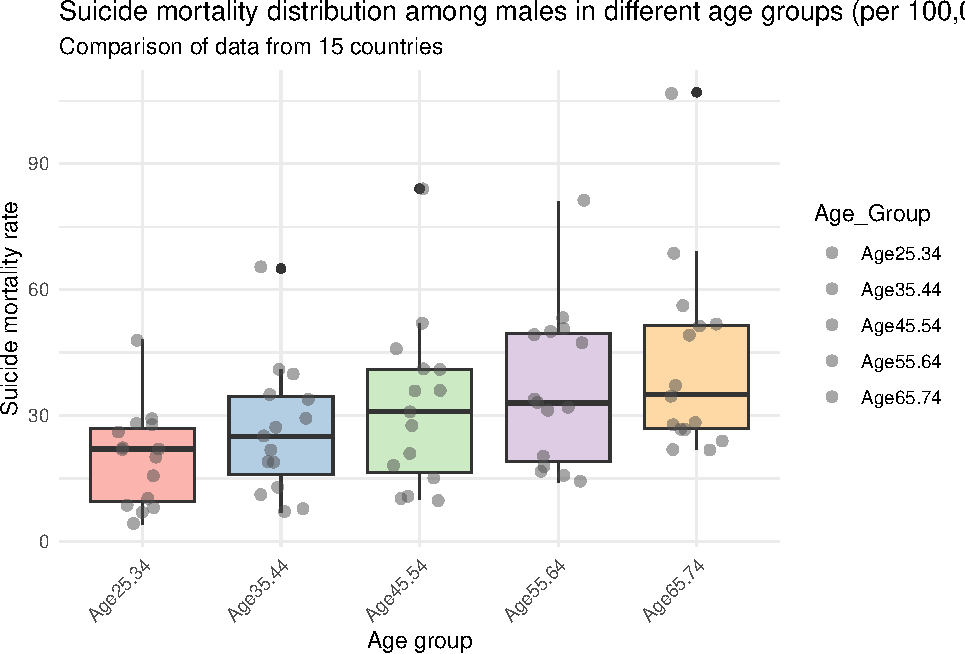
\includegraphics{final2025_files/figure-latex/unnamed-chunk-22-1.pdf}

\begin{Shaded}
\begin{Highlighting}[]
\CommentTok{\# 分析数据}
\FunctionTok{cat}\NormalTok{(}\StringTok{"}\SpecialCharTok{\textbackslash{}n}\StringTok{数据分析:}\SpecialCharTok{\textbackslash{}n}\StringTok{"}\NormalTok{)}
\end{Highlighting}
\end{Shaded}

\begin{verbatim}
## 
## 数据分析:
\end{verbatim}

\begin{Shaded}
\begin{Highlighting}[]
\FunctionTok{cat}\NormalTok{(}\StringTok{"1. 死亡率随年龄增长而上升: 从25{-}34岁组到55{-}64岁组，死亡率中位数持续增加}\SpecialCharTok{\textbackslash{}n}\StringTok{"}\NormalTok{)}
\end{Highlighting}
\end{Shaded}

\begin{verbatim}
## 1. 死亡率随年龄增长而上升: 从25-34岁组到55-64岁组，死亡率中位数持续增加
\end{verbatim}

\begin{Shaded}
\begin{Highlighting}[]
\FunctionTok{cat}\NormalTok{(}\StringTok{"2. 最高死亡率在65{-}74岁组: 该组死亡率中位数最高，且分布范围最广}\SpecialCharTok{\textbackslash{}n}\StringTok{"}\NormalTok{)}
\end{Highlighting}
\end{Shaded}

\begin{verbatim}
## 2. 最高死亡率在65-74岁组: 该组死亡率中位数最高，且分布范围最广
\end{verbatim}

\begin{Shaded}
\begin{Highlighting}[]
\FunctionTok{cat}\NormalTok{(}\StringTok{"3. 变异程度随年龄增加: 老年组(55{-}64岁和65{-}74岁)的数据范围更大，显示国家间差异更显著}\SpecialCharTok{\textbackslash{}n}\StringTok{"}\NormalTok{)}
\end{Highlighting}
\end{Shaded}

\begin{verbatim}
## 3. 变异程度随年龄增加: 老年组(55-64岁和65-74岁)的数据范围更大，显示国家间差异更显著
\end{verbatim}

\begin{Shaded}
\begin{Highlighting}[]
\FunctionTok{cat}\NormalTok{(}\StringTok{"4. 离群点: 在65{-}74岁组观察到极高值(\textgreater{}100)，可能是匈牙利的数据}\SpecialCharTok{\textbackslash{}n}\StringTok{"}\NormalTok{)}
\end{Highlighting}
\end{Shaded}

\begin{verbatim}
## 4. 离群点: 在65-74岁组观察到极高值(>100)，可能是匈牙利的数据
\end{verbatim}

\begin{Shaded}
\begin{Highlighting}[]
\FunctionTok{cat}\NormalTok{(}\StringTok{"5. 最低死亡率在年轻组: 25{-}34岁组整体死亡率最低，但国家间差异明显}\SpecialCharTok{\textbackslash{}n}\StringTok{"}\NormalTok{)}
\end{Highlighting}
\end{Shaded}

\begin{verbatim}
## 5. 最低死亡率在年轻组: 25-34岁组整体死亡率最低，但国家间差异明显
\end{verbatim}

\begin{Shaded}
\begin{Highlighting}[]
\CommentTok{\# 计算各年龄组统计量}
\NormalTok{age\_group\_stats }\OtherTok{\textless{}{-}}\NormalTok{ suicrates\_long }\SpecialCharTok{\%\textgreater{}\%}
  \FunctionTok{group\_by}\NormalTok{(Age\_Group) }\SpecialCharTok{\%\textgreater{}\%}
  \FunctionTok{summarise}\NormalTok{(}
    \AttributeTok{Median =} \FunctionTok{median}\NormalTok{(Mortality\_Rate),}
    \AttributeTok{Mean =} \FunctionTok{mean}\NormalTok{(Mortality\_Rate),}
    \AttributeTok{SD =} \FunctionTok{sd}\NormalTok{(Mortality\_Rate),}
    \AttributeTok{Min =} \FunctionTok{min}\NormalTok{(Mortality\_Rate),}
    \AttributeTok{Max =} \FunctionTok{max}\NormalTok{(Mortality\_Rate)}
\NormalTok{  )}

\FunctionTok{cat}\NormalTok{(}\StringTok{"}\SpecialCharTok{\textbackslash{}n}\StringTok{各年龄组统计摘要:}\SpecialCharTok{\textbackslash{}n}\StringTok{"}\NormalTok{)}
\end{Highlighting}
\end{Shaded}

\begin{verbatim}
## 
## 各年龄组统计摘要:
\end{verbatim}

\begin{Shaded}
\begin{Highlighting}[]
\FunctionTok{print}\NormalTok{(age\_group\_stats)}
\end{Highlighting}
\end{Shaded}

\begin{verbatim}
## # A tibble: 5 x 6
##   Age_Group Median  Mean    SD   Min   Max
##   <chr>      <dbl> <dbl> <dbl> <dbl> <dbl>
## 1 Age25.34      22  19.9  11.5     4    48
## 2 Age35.44      25  26.3  15.3     7    65
## 3 Age45.54      31  32    19.9    10    84
## 4 Age55.64      33  36.4  18.7    14    81
## 5 Age65.74      35  42.3  23.0    22   107
\end{verbatim}

\subsection{7.}\label{section-6}

Load the \texttt{LaborSupply} dataset from the \texttt{\{Ecdat\}}
package and answer the following questions:

\begin{Shaded}
\begin{Highlighting}[]
\CommentTok{\#data(LaborSupply)}
\NormalTok{LaborSupply }\OtherTok{\textless{}{-}} \FunctionTok{read\_csv}\NormalTok{(}\StringTok{"LaborSupply.csv"}\NormalTok{)}
\end{Highlighting}
\end{Shaded}

\begin{verbatim}
## Rows: 5320 Columns: 7
## -- Column specification --------------------------------------------------------
## Delimiter: ","
## dbl (7): lnhr, lnwg, kids, age, disab, id, year
## 
## i Use `spec()` to retrieve the full column specification for this data.
## i Specify the column types or set `show_col_types = FALSE` to quiet this message.
\end{verbatim}

\begin{Shaded}
\begin{Highlighting}[]
\CommentTok{\# create hour and wage variables}
\NormalTok{labor }\OtherTok{\textless{}{-}}\NormalTok{ LaborSupply }\SpecialCharTok{|\textgreater{}} 
  \FunctionTok{mutate}\NormalTok{(}\AttributeTok{hour =} \FunctionTok{exp}\NormalTok{(lnhr), }\AttributeTok{wage =} \FunctionTok{exp}\NormalTok{(lnwg), }\AttributeTok{.before =}\NormalTok{ kids) }\SpecialCharTok{|\textgreater{}} 
\NormalTok{  dplyr}\SpecialCharTok{::}\FunctionTok{select}\NormalTok{(}\SpecialCharTok{{-}}\NormalTok{lnhr, }\SpecialCharTok{{-}}\NormalTok{lnwg)}
\end{Highlighting}
\end{Shaded}

\begin{enumerate}
\def\labelenumi{\alph{enumi}.}
\tightlist
\item
  Compute the average annual hours worked and their standard deviations
  by year.
\end{enumerate}

\begin{Shaded}
\begin{Highlighting}[]
\NormalTok{hourly\_stats }\OtherTok{\textless{}{-}}\NormalTok{ labor }\SpecialCharTok{\%\textgreater{}\%}
  \FunctionTok{group\_by}\NormalTok{(year) }\SpecialCharTok{\%\textgreater{}\%}
  \FunctionTok{summarise}\NormalTok{(}
    \AttributeTok{avg\_hours =} \FunctionTok{mean}\NormalTok{(hour, }\AttributeTok{na.rm =} \ConstantTok{TRUE}\NormalTok{),}
    \AttributeTok{sd\_hours =} \FunctionTok{sd}\NormalTok{(hour, }\AttributeTok{na.rm =} \ConstantTok{TRUE}\NormalTok{)}
\NormalTok{  )}

\FunctionTok{cat}\NormalTok{(}\StringTok{"a. 按年份的平均工作小时数及标准差:}\SpecialCharTok{\textbackslash{}n}\StringTok{"}\NormalTok{)}
\end{Highlighting}
\end{Shaded}

\begin{verbatim}
## a. 按年份的平均工作小时数及标准差:
\end{verbatim}

\begin{Shaded}
\begin{Highlighting}[]
\FunctionTok{print}\NormalTok{(hourly\_stats)}
\end{Highlighting}
\end{Shaded}

\begin{verbatim}
## # A tibble: 10 x 3
##     year avg_hours sd_hours
##    <dbl>     <dbl>    <dbl>
##  1  1979     2202.     502.
##  2  1980     2182.     454.
##  3  1981     2185.     460.
##  4  1982     2145.     442.
##  5  1983     2124.     550.
##  6  1984     2149.     492.
##  7  1985     2203.     515.
##  8  1986     2195.     482.
##  9  1987     2219.     529.
## 10  1988     2222.     478.
\end{verbatim}

\begin{enumerate}
\def\labelenumi{\alph{enumi}.}
\setcounter{enumi}{1}
\tightlist
\item
  What age group worked the most hours in the year 1982?
\end{enumerate}

\begin{Shaded}
\begin{Highlighting}[]
\NormalTok{age\_group\_1982 }\OtherTok{\textless{}{-}}\NormalTok{ labor }\SpecialCharTok{|\textgreater{}}
\FunctionTok{filter}\NormalTok{(year }\SpecialCharTok{==} \DecValTok{1982}\NormalTok{) }\SpecialCharTok{|\textgreater{}}
\FunctionTok{group\_by}\NormalTok{(age) }\SpecialCharTok{|\textgreater{}}
  \FunctionTok{summarise}\NormalTok{(}\AttributeTok{avg\_hours =} \FunctionTok{mean}\NormalTok{(hour)) }\SpecialCharTok{|\textgreater{}}
\FunctionTok{arrange}\NormalTok{(}\FunctionTok{desc}\NormalTok{(avg\_hours)) }\SpecialCharTok{|\textgreater{}}
\FunctionTok{slice}\NormalTok{(}\DecValTok{1}\NormalTok{)}
\FunctionTok{cat}\NormalTok{(}\StringTok{" 年龄:"}\NormalTok{, age\_group\_1982}\SpecialCharTok{$}\NormalTok{age, }\StringTok{" 岁 | 平均工作时长:"}\NormalTok{, }\FunctionTok{round}\NormalTok{(age\_group\_1982}\SpecialCharTok{$}\NormalTok{avg\_hours, }\DecValTok{1}\NormalTok{), }\StringTok{" 小时}\SpecialCharTok{\textbackslash{}n}\StringTok{"}\NormalTok{)}
\end{Highlighting}
\end{Shaded}

\begin{verbatim}
##  年龄: 46  岁 | 平均工作时长: 2373.5  小时
\end{verbatim}

\begin{enumerate}
\def\labelenumi{\alph{enumi}.}
\setcounter{enumi}{2}
\tightlist
\item
  Create a variable, \texttt{n\_years} that equals the number of years
  an individual stays in the panel. Is the panel balanced?
\end{enumerate}

\begin{Shaded}
\begin{Highlighting}[]
\CommentTok{\# 计算每个个体参与的年数}
\NormalTok{n\_years }\OtherTok{\textless{}{-}}\NormalTok{ labor }\SpecialCharTok{\%\textgreater{}\%}
  \FunctionTok{group\_by}\NormalTok{(id) }\SpecialCharTok{\%\textgreater{}\%}
  \FunctionTok{summarise}\NormalTok{(}\AttributeTok{n\_years =} \FunctionTok{n\_distinct}\NormalTok{(year))}

\CommentTok{\# 添加到主数据集}
\NormalTok{labor }\OtherTok{\textless{}{-}}\NormalTok{ labor }\SpecialCharTok{\%\textgreater{}\%}
  \FunctionTok{left\_join}\NormalTok{(n\_years, }\AttributeTok{by =} \StringTok{"id"}\NormalTok{)}

\CommentTok{\# 检查面板是否平衡}
\NormalTok{is\_balanced }\OtherTok{\textless{}{-}} \FunctionTok{all}\NormalTok{(n\_years}\SpecialCharTok{$}\NormalTok{n\_years }\SpecialCharTok{==} \FunctionTok{max}\NormalTok{(n\_years}\SpecialCharTok{$}\NormalTok{n\_years))}
\FunctionTok{cat}\NormalTok{(}\StringTok{"}\SpecialCharTok{\textbackslash{}n}\StringTok{c. 面板是否平衡?"}\NormalTok{, }\FunctionTok{ifelse}\NormalTok{(is\_balanced, }\StringTok{"是"}\NormalTok{, }\StringTok{"否"}\NormalTok{), }\StringTok{"}\SpecialCharTok{\textbackslash{}n}\StringTok{"}\NormalTok{)}
\end{Highlighting}
\end{Shaded}

\begin{verbatim}
## 
## c. 面板是否平衡? 是
\end{verbatim}

\begin{Shaded}
\begin{Highlighting}[]
\FunctionTok{cat}\NormalTok{(}\StringTok{"   每个个体参与的年数范围:"}\NormalTok{, }\FunctionTok{range}\NormalTok{(n\_years}\SpecialCharTok{$}\NormalTok{n\_years), }\StringTok{"}\SpecialCharTok{\textbackslash{}n}\StringTok{"}\NormalTok{)}
\end{Highlighting}
\end{Shaded}

\begin{verbatim}
##    每个个体参与的年数范围: 10 10
\end{verbatim}

\begin{enumerate}
\def\labelenumi{\alph{enumi}.}
\setcounter{enumi}{3}
\tightlist
\item
  Which are the individuals that do not have any kids during the whole
  period? Create a variable, \texttt{no\_kids}, that flags these
  individuals (1 = no kids, 0 = kids)
\end{enumerate}

\begin{Shaded}
\begin{Highlighting}[]
\CommentTok{\# 找出整个期间都没有子女的个体}
\NormalTok{no\_kids\_ids }\OtherTok{\textless{}{-}}\NormalTok{ labor }\SpecialCharTok{\%\textgreater{}\%}
  \FunctionTok{group\_by}\NormalTok{(id) }\SpecialCharTok{\%\textgreater{}\%}
  \FunctionTok{summarise}\NormalTok{(}\AttributeTok{always\_no\_kids =} \FunctionTok{all}\NormalTok{(kids }\SpecialCharTok{==} \DecValTok{0}\NormalTok{)) }\SpecialCharTok{\%\textgreater{}\%}
  \FunctionTok{filter}\NormalTok{(always\_no\_kids) }\SpecialCharTok{\%\textgreater{}\%}
  \FunctionTok{pull}\NormalTok{(id)}

\CommentTok{\# 创建no\_kids变量}
\NormalTok{labor }\OtherTok{\textless{}{-}}\NormalTok{ labor }\SpecialCharTok{\%\textgreater{}\%}
  \FunctionTok{mutate}\NormalTok{(}\AttributeTok{no\_kids =} \FunctionTok{if\_else}\NormalTok{(id }\SpecialCharTok{\%in\%}\NormalTok{ no\_kids\_ids, }\DecValTok{1}\NormalTok{, }\DecValTok{0}\NormalTok{))}

\FunctionTok{cat}\NormalTok{(}\StringTok{"}\SpecialCharTok{\textbackslash{}n}\StringTok{d. 整个期间无子女的个体数量:"}\NormalTok{, }\FunctionTok{length}\NormalTok{(no\_kids\_ids), }\StringTok{"}\SpecialCharTok{\textbackslash{}n}\StringTok{"}\NormalTok{)}
\end{Highlighting}
\end{Shaded}

\begin{verbatim}
## 
## d. 整个期间无子女的个体数量: 43
\end{verbatim}

\begin{enumerate}
\def\labelenumi{\alph{enumi}.}
\setcounter{enumi}{4}
\tightlist
\item
  Using the \texttt{no\_kids} variable from before compute the average
  wage, standard deviation and number of observations in each group for
  the year 1980 (no kids group vs kids group).
\end{enumerate}

\begin{Shaded}
\begin{Highlighting}[]
\CommentTok{\# e. 1980年按有无子女分组的工资统计}
\NormalTok{wage\_stats\_1980 }\OtherTok{\textless{}{-}}\NormalTok{ labor }\SpecialCharTok{\%\textgreater{}\%}
  \FunctionTok{filter}\NormalTok{(year }\SpecialCharTok{==} \DecValTok{1980}\NormalTok{) }\SpecialCharTok{\%\textgreater{}\%}
  \FunctionTok{group\_by}\NormalTok{(no\_kids) }\SpecialCharTok{\%\textgreater{}\%}
  \FunctionTok{summarise}\NormalTok{(}
    \AttributeTok{avg\_wage =} \FunctionTok{mean}\NormalTok{(wage, }\AttributeTok{na.rm =} \ConstantTok{TRUE}\NormalTok{),}
    \AttributeTok{sd\_wage =} \FunctionTok{sd}\NormalTok{(wage, }\AttributeTok{na.rm =} \ConstantTok{TRUE}\NormalTok{),}
    \AttributeTok{n\_obs =} \FunctionTok{n}\NormalTok{()}
\NormalTok{  ) }\SpecialCharTok{\%\textgreater{}\%}
  \FunctionTok{mutate}\NormalTok{(}\AttributeTok{no\_kids =} \FunctionTok{factor}\NormalTok{(no\_kids, }\AttributeTok{labels =} \FunctionTok{c}\NormalTok{(}\StringTok{"有子女"}\NormalTok{, }\StringTok{"无子女"}\NormalTok{)))}

\FunctionTok{cat}\NormalTok{(}\StringTok{"}\SpecialCharTok{\textbackslash{}n}\StringTok{e. 1980年按有无子女分组的工资统计:}\SpecialCharTok{\textbackslash{}n}\StringTok{"}\NormalTok{)}
\end{Highlighting}
\end{Shaded}

\begin{verbatim}
## 
## e. 1980年按有无子女分组的工资统计:
\end{verbatim}

\begin{Shaded}
\begin{Highlighting}[]
\FunctionTok{print}\NormalTok{(wage\_stats\_1980)}
\end{Highlighting}
\end{Shaded}

\begin{verbatim}
## # A tibble: 2 x 4
##   no_kids avg_wage sd_wage n_obs
##   <fct>      <dbl>   <dbl> <int>
## 1 有子女      14.5    6.69   489
## 2 无子女      15.9    6.71    43
\end{verbatim}

\end{document}
